\documentclass[sigplan,nonacm,10pt]{acmart}

%% The frontier paper (FRONTIER-PLAN.md §4): a NEW submission, not a
%% version of "Untrusted Authors, Trusted Answers" — the map is the
%% contribution and the calculus is cited as the means (the instrument
%% paper, arXiv v2 — tag arxiv.2). All sections are written in
%% lockstep with mechanization/Calculus/Frontier.lean. The paper
%% deliberately carries no measurements section: §7
%% (sections/status.tex) summarizes where the experiments stand — the
%% seven-iteration hwmcc-sosylab-beem campaign, every number read from
%% the deposited ledger in ../results/ — and §8 (sections/vision.tex)
%% states the staged discovery program (INVERSION.md, distilled). The
%% full iteration-by-iteration saturation report that previously stood
%% as §7 is preserved in git history (sections/benchmarks.tex at
%% a0bb1ee/343cd5a) and regenerates from the ledger.
%%
%% From-scratch preamble on purpose: this document shares only
%% ../references.bib with the instrument paper. Everything the
%% instrument paper's macros provide and this paper does not use is
%% pruned.
\settopmatter{printfolios=true,printccs=false,printacmref=false}
\pagestyle{plain}

\usepackage{booktabs}
\usepackage{xspace}
\usepackage{tikz}
\usetikzlibrary{positioning,arrows.meta,calc}

\newcommand{\hg}{hurdy-gurdy\xspace}
%% The five conditions, in diagnosis order — one macro so the order is
%% typeset identically everywhere.
\newcommand{\obstacles}{connectivity, loss, shape, cost, trust\xspace}

%% acmart loads amsthm and defines theorem/lemma/definition/etc.
\theoremstyle{definition}
\newtheorem{assumption}{Assumption}
\usepackage[capitalise]{cleveref}
\crefname{assumption}{assumption}{assumptions}
\Crefname{assumption}{Assumption}{Assumptions}

\emergencystretch=1.5em

\begin{document}

\title{The hurdy-gurdy Platform}
\subtitle{Exploring the Frontier of Reducible Decidability in Practice}

\author{Christoph Kirsch}
\affiliation{%
  \institution{University of Salzburg, Austria}\country{}}
\affiliation{%
  \institution{Czech Technical University, Prague, Czechia}\country{}}
\email{ck@cs.uni-salzburg.at}

\begin{abstract}
We are constructing a platform for exploring the \emph{frontier of
reducible decidability in practice} --- which questions about
programs can be answered, today, by chains of sound reductions to
mechanized decision procedures within declared budgets --- and,
eventually, for pushing it. The method is \emph{saturation}: present
the platform a pinned benchmark and run it until every question is
either answered along every feasible route, with measured cost and
quantified trust, or open on the books with its first failing
obstacle and the exact missing instrument --- a \emph{frontier pair}
whose required contract is derived mechanically --- or the stated
reason none can. Each saturation deposits a map, and the maps
compound. Throughout, LLMs both \emph{deploy} \hg{} and
\emph{develop} it --- playing the questions, and building the
translation pairs and, in a gated shadow lane, the decision
procedures the books demand --- with user intervention minimized to
one act, the valve: registering what may be built, or writing the
mandate that delegates that registration. The architecture is what
makes this safe: untrusted authors, trusted
answers~\citep{hurdygurdy2026calculus}. We state six facilitation
theorems with their honest assumptions --- exploration is sound (the
map cannot be falsified by its untrusted explorer), monotone,
self-directing, relatively complete in the lineage of Cook,
terminating per benchmark, and domain-generic --- with the
compositional core mechanized in Lean~4, and the domain kit a field
must supply. The pre-registered protocol has now run its first
campaign, seven loop iterations over a pinned hardware
model-checking suite; this paper carries no measurements section,
only a summary of where the experiments stand, because the campaign's
structural lesson matters more than its numbers: a loop whose every
artifact is meaning-preserving is conservative over truth --- it
discovers instruments, never facts. We close with the program that
lifts that ceiling: the platform is one equation solved for one
unknown, and the same equation solved for its other unknowns is
property, abstraction, semantics, and procedure discovery, each
checked by the gate that already exists.
\end{abstract}

\maketitle

%% §1 — re-cut 2026-08-06 for the kernel architecture (KERNEL.md).
%% The Era-3 introduction (filtration, six theorems, valve) is in git
%% history at 4b17542 and summarized in HISTORY.md.

\section{Introduction}
\label{sec:intro}

We are interested in constructing a platform that enables us to
explore the frontier of \emph{reducible decidability in practice} ---
and, eventually, to push it. The phrase is chosen word by word. A
question about a program is \emph{reducibly decidable} when some
finite chain of checked reductions carries it to a mechanized
decision procedure that answers it; the reachable set is the closure
of the questions under the reductions one actually has, not an
oracle's reach. And \emph{in practice} means within declared budgets,
measured and never asymptotic: a procedure that exceeds every budget
is not a way, and where that boundary lies is an empirical fact that
moves with every solver, abstraction, and logic the world supplies.
The frontier, so understood, is a real and interesting object: on its
near side, everything formal methods can do today, enumerated and
priced; on its far side, structured evidence about exactly what is
missing.

An earlier design of \hg{} explored this frontier as a cartography
problem, with a five-condition answerability filtration, a typed
demand ledger, six facilitation theorems, and a human registration
valve; its calculus and measured snapshot are the subject of a
companion paper~\citep{hurdygurdy2026calculus}, and its first
campaign ran to completion (\cref{sec:status}). The campaign taught
two lessons. Structurally: a loop whose every admissible artifact is
meaning-preserving is \emph{conservative over truth} --- it discovers
instruments, never facts --- so after seven iterations over a suite
native to its best solver, the loop's entire demand output read
\emph{get a better engine}. And architecturally: the machinery that
tracked demand --- books, boards, briefs, mandates, lanes, the
filtration --- had each earned its place and jointly grown past its
justification, because its consumer changed. Demand used to feed
mechanical derivation, which needs typed taxonomies; it now feeds an
LLM conjecturing, which wants rich evidence and tolerates prose.

This paper describes the platform designed fresh from those lessons,
around one organizing move:

\begin{quote}
\textbf{Translation and solving are the same kind of edge, and
results are the only currency.}
\end{quote}

A \emph{solver pair} is a pair whose target is the language of
results: translating \emph{is} solving under a declared budget
(\cref{sec:kernel}). A \emph{result} is a replayed witness, a
universal claim up to a bound (or unbounded, with a certificate), or
an honest \emph{partial} --- a description of how far a route got and
where it failed. The \emph{frontier of a benchmark} is exactly the
set of its questions whose best result is not terminal
(\cref{sec:map}) --- no separate bookkeeping for failure exists. An
LLM plays a pinned benchmark autonomously until a human pulls the
plug, conjecturing in a fixed order that is the vision's core
discipline --- new decision procedures first, then new translations,
then new languages: \emph{semantics first, then syntax}
(\cref{sec:loop}) --- and everything it builds passes one gate. The
trust story is one sentence: \textbf{the LLM never writes a result;
only the kernel does, by running checked code.}

The kernel --- the fixed, hand-written part --- is deliberately small
enough to read in an afternoon, and its properties are mechanized in
Lean~4: the result order is strict, best-per-question is a ratchet
under log growth, terminal questions stay terminal, grades only climb
(\cref{sec:proofs}). Everything else is generated content admitted
through the gate, and the previous generation of the platform is the
first such content: its languages, pairs, and engines are carried
over by wrapping them in kernel manifests and re-certifying them
through the gate they must now pass (\cref{sec:status}).

\paragraph{Contributions}
\begin{itemize}
\item One edge kind: solver pairs as translation into a result
  language, with the commuting square degenerating to result
  validity, so translations and decision procedures share one
  admission gate (\cref{sec:kernel}).
\item Results as the only currency: a fixed result schema whose
  order (level, bound, grade) makes the frontier a derived object ---
  the non-terminal best results --- and monotone exploration a
  property of the data structure, not a theorem apparatus
  (\cref{sec:map}).
\item The certification symmetry: both existential and universal
  answers are carry-back-then-check, witness replay mirrored by
  certificate re-discharge, with a strict grade ladder
  \emph{claimed} $<$ \emph{checked} $<$ \emph{certified} whose top
  rung is reserved for route-independent evidence
  (\cref{sec:cert}).
\item The autonomous loop: no registration valve, one gate with
  measured determinism and two-sided controls, a fixed
  semantics-first conjecture order, plug-pull safety at any moment,
  and bootstrap from an empty instance (\cref{sec:loop}).
\item The kernel mechanized, and an honest accounting of the
  previous design: where each of its six facilitation theorems went
  --- proved smaller, made structural, or retired with the machinery
  that needed it (\cref{sec:proofs}).
\item Exactly the experiments the redesign rests on: the campaign
  that forced it, and the carried-over demonstration whose
  three-question map reproduces the campaign's structural finding in
  miniature (\cref{sec:status}).
\end{itemize}

%% §2 — the frontier problem. Drafted in Phase 1, in lockstep with
%% mechanization/Calculus/Frontier.lean: every definition below is the
%% Lean definition, prose first. This section is the paper's
%% contribution of *problem* and must stand alone.

\section{The frontier problem}
\label{sec:problem}

\paragraph{Domains}
A \emph{domain} is where questions live and decisions happen. Its
signature supplies, and nothing else about it matters:
languages, each carrying a \emph{formal semantics} --- a definable
meaning function over its programs, exposing named \emph{observables}
--- with formal semantics the only admission criterion; among them
some \emph{reasoning languages}, each owning mechanized decision
procedures with declared budgets and, where available, certificate
checkers; and a supply of independent \emph{semantic anchors} ---
external formalizations against which a translation can be checked by
something its author did not write. Hardware model checking is a
domain; C program analysis is a domain; chemical reaction networks
are a domain. The theorems of \Cref{sec:theorems} use only the
signature, which is what \emph{in any given domain} will mean.

\paragraph{Questions}
A \emph{question} $q = (p, \varphi)$ is a program $p$ in one of the
domain's languages and a condition $\varphi$ over $p$'s observables,
asked existentially (is $\varphi$ reachable?) or universally (does
$\varphi$ hold for all inputs, within declared bounds?). A
\emph{benchmark} $B$ is a pinned, finite set of questions with
recorded provenance --- pinned, so that ``the benchmark'' names the
same set at every loop iteration.

\paragraph{Items, registries, candidates}
The unit of admission is the \emph{item}: either a \emph{pair} --- a
deterministic, contract-carrying translation edge between two
languages~\citep{hurdygurdy2026calculus} --- or a language-attached
\emph{capability}: a solver, a checker, an anchor. A \emph{registry}
$G$ is the set of admitted items; growth is additive (items are
admitted, never silently removed), and every admission is gated. A
\emph{candidate} answer for $q$ rests on finitely many items: the
route's hops plus the destination capabilities it invokes --- one
list. Pairs for edges, capabilities for nodes: a candidate is the
route-level object, and it is the only object the definitions below
need.

\begin{definition}[Answerability]
\label{def:answerable}
Fix, per domain, $N$ \emph{conditions} on candidates, checked in a
fixed \emph{diagnosis order}. \hg{} instantiates $N = 5$:
\emph{connectivity} (the candidate is a route from $p$'s language to
a reasoning language), \emph{loss} ($\varphi$'s observables survive
the route's composed projection), \emph{shape} ($\varphi$'s logical
form is one the destination's procedures decide), \emph{cost} (a
procedure returns a verdict other than
\textit{unknown}/\textit{resource-out} within its declared budget),
and \emph{trust} (the answer meets the asker's assurance floor).
Write $S_k(G, q)$ for the candidates available in $G$ that survive
the first $k$ conditions --- the \emph{answerability filtration},
shrinking as $k$ grows and growing as $G$ grows. Then $q$ is
\emph{answerable at $G$} iff $S_N(G, q) \neq \emptyset$.
\end{definition}

Two words in the title are fixed by this definition.
\emph{In practice}: the cost condition quantifies over declared
budgets and measured runs, never over asymptotics ---
\textit{resource-out} is a permanent verdict class, and a route
without a measurement reads \textit{unmeasured}, never cheap.
\emph{Reducible}: answerability quantifies over candidates built from
admitted items, so the answerable set is the closure of the domain's
questions under the admitted reductions --- not an oracle's reach.

\begin{definition}[Diagnosis]
\label{def:diagnosis}
For $q$ unanswerable at $G$, the \emph{diagnosis} is the first
failing condition: the $k$ with $S_k(G,q) \neq \emptyset =
S_{k+1}(G,q)$. \Cref{thm:gradient} shows it exists, is unique, and
under growth only advances --- ``the obstacle'' is honest vocabulary,
and it is the frontier's local gradient: which kind of instrument
would move the map \emph{here}.
\end{definition}

\paragraph{The currency: three tiers of pair}
A pair carries a \emph{contract}: its assurance class, the direction
of its square, its kept observables, its measured
cost~\citep{hurdygurdy2026calculus}. Contracts compose along a route
by the componentwise meet and are ordered by strength; the meet is
what makes the following duality compose.

\begin{definition}[Required and achieved contracts; the tiers]
\label{def:tiers}
An implemented pair carries an \emph{achieved} contract, verified
from above: evidence establishes \emph{at least this}. A
\emph{frontier pair} carries a \emph{required} contract, demanded
from below: the join, over the open questions that cite it, of the
observables they need kept, the direction and assurance they need,
with cost kept as the histogram of their budgets. It also carries its
\emph{design evidence} --- everything the books know about how to get
there (\Cref{sec:kit}) --- and, where the demanded target is a
reasoning language that does not exist, a \emph{hypothetical}
endpoint: a language sketch, a typed hole in the graph. The registry
thus holds one lifecycle in three tiers:
\[
\textit{frontier} \;\longrightarrow\; \textit{registered}
\;\longrightarrow\; \textit{partial} \rightarrow \textit{built},
\]
where \emph{frontier} means design unknown, \emph{registered} means a
human admitted a design (the brief's ``intended translator'' is
filled in), and \emph{partial}/\emph{built} mean an achieved,
measured contract. Registering a frontier pair \emph{means}
exhibiting a design whose achievable contract dominates the required
one; promotion only ever advances, and the evidence payload travels
(\Cref{thm:currency}).
\end{definition}

Demand is not only edge-shaped. A missing \emph{capability} --- a
decision procedure no registered hub supplies --- is demanded in the
same currency, and a curated atlas of the known decidability
landscape (\Cref{sec:kit}) draws its line against the known set: a
\emph{charted} procedure family (setting, family, and canonical
crossings known) lies inside --- instantiation, and it blocks
saturation honestly --- while an \emph{uncharted} shape lies outside,
labeled discovery, never a guess.

\begin{definition}[Conditional routes]
\label{def:conditional}
A route may mix implemented and frontier hops. Its \emph{conditional
contract} is the meet over all hops --- achieved contracts for
implemented hops, required contracts for frontier hops --- and it is
read as: \emph{if} each frontier hop is discharged by a pair
achieving its requirement, this route answers $q$ with at least this
contract. Conditional routes are never executable; they are the
plan-shaped reading of the map, and \Cref{thm:currency} is what makes
them sound.
\end{definition}

\begin{definition}[Saturation]
\label{def:saturation}
$B$ is \emph{saturated at $G$} when the pair-shaped demand its open
questions derive contains no \emph{registered-able} candidate over
the known set --- no tier-2 design over the registered languages,
solvers, and anchors would add a feasible way, a cheaper way, or a
more trusted way --- i.e., every question in $B$ is in one of two
terminal states: \emph{solved, all ways}, its answer carrying the
census of every feasible route with measured cost profile, assurance
class, and corroboration; or \emph{open, on the books}, its frontier
pairs (if any are honest to name) all lying outside the known set,
partitioned by obstacle. Saturation is an emptiness check on a
derived set --- mechanically detectable, no judgment call --- and it
is \emph{reopened only by good news}: a new solver, anchor, or logic
re-enters the known set exactly where the terminal board says it
plugs in.
\end{definition}

\paragraph{The map}
The deliverable of saturating $B$ is its \emph{map}: the answered
fraction of $B$ per loop iteration (monotone, by
\Cref{thm:monotone}); cost per answer across iterations; per solved
question, the way-census; and the \emph{terminal board} --- the
surviving frontier pairs with their obstacle partition, required
contracts, design evidence, and distinct-question counts. The board
is the domain's future-work section, machine-generated; the map is
drawn in the same currency the instrument is built from.

%% §3 — written out in Phase 4. The requirement-table spine: each
%% feature of the instrument stated as the requirement of trustworthy
%% cartography it serves. Details and proofs live in
%% \citep{hurdygurdy2026calculus} and the Lean; nothing is re-derived.

\section{The instrument, as means}
\label{sec:instrument}

None of \hg's load-bearing features was designed as a feature of one
more verification tool. Read from the story's end, each is a
requirement of frontier cartography — what it takes for the maps of
\Cref{sec:problem} to be worth keeping:

\begin{center}
\footnotesize
\begin{tabular}{@{}ll@{}}
\toprule
a trustworthy map needs\ldots & supplied by \\
\midrule
labels its explorer cannot falsify & determinism + the square (\S\ref{sec:inst-pairs}) \\
composition told honestly, once & the contract meet (\S\ref{sec:inst-contracts}) \\
untrusted authors, trusted answers & the asymmetry (\S\ref{sec:inst-asym}) \\
ground that is never lost & the gate and the ratchet (\S\ref{sec:inst-gate}) \\
the far side, saved as evidence & the books, on two planes (\S\ref{sec:inst-gate}) \\
\bottomrule
\end{tabular}
\end{center}

\subsection{Pairs and the directional square}
\label{sec:inst-pairs}

The unit is the \emph{pair}: two languages with formal semantics, a
pure translator $T$, pure shared interpreters $I_s, I_t$, and a pure
target-to-source interpreter $\Lambda$ carrying target behaviors back
to source vocabulary. These close a commuting square
(\Cref{fig:square}),
$I_s(p) \equiv_\pi \Lambda(I_t(T(p)))$, up to a declared projection
$\pi$ — the observables the pair promises to preserve — and the
square is \emph{directional}: an abstraction pair declares
$\sqsubseteq_\pi$ instead (every source behavior has a target
counterpart; the target may deliberately have more) and ships a
witness embedding along which its lax square is checked exactly like
an exact one. The square is decidable \emph{per program}: run both
sides, compare under $\pi$, and a failure names its step and
observable. That per-program decidability, resting on determinism
(same input, byte-identical output, always), is what makes the map's
solved region checkable rather than asserted: every entry can be
re-derived, and a defect points at itself. Squares paste, so pairs
compose into \emph{routes} through the registry
graph~\citep{hurdygurdy2026calculus}.

\begin{figure}
\centering
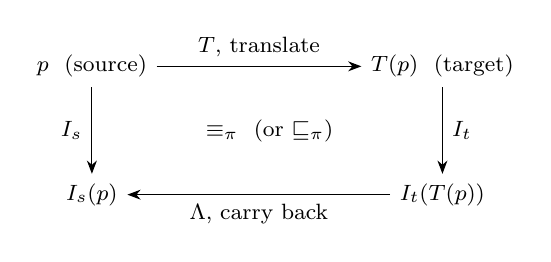
\begin{tikzpicture}[font=\footnotesize, >=Stealth,
  node distance=11mm and 26mm]
  \node (p)  {$p$ \ (source)};
  \node[right=of p]  (tp) {$T(p)$ \ (target)};
  \node[below=of p]  (sb) {$I_s(p)$};
  \node[below=of tp] (tb) {$I_t(T(p))$};
  \draw[->] (p)  -- node[above] {$T$, translate} (tp);
  \draw[->] (p)  -- node[left]  {$I_s$} (sb);
  \draw[->] (tp) -- node[right] {$I_t$} (tb);
  \draw[->] (tb) -- node[below] {$\Lambda$, carry back} (sb);
  \path (p) -- node[midway] {$\equiv_\pi$ \ (or $\sqsubseteq_\pi$)} (tb);
\end{tikzpicture}
\caption{The pair as a commuting square: interpreting the source
directly agrees, on the declared projection $\pi$, with translating,
interpreting the translation, and carrying the behavior back. A
directional (abstraction) pair declares $\sqsubseteq_\pi$ instead
and ships a witness embedding along which the lax square is checked
exactly; a failure localizes to a step and an observable.}
\label{fig:square}
\end{figure}

\subsection{Contracts and the meet}
\label{sec:inst-contracts}

A pair's composable declaration is its \emph{contract}: assurance
class, direction, kept observables, measured cost. Contracts compose
along a route by the componentwise meet — the weakest hop on every
axis at once, mechanized as \textsf{Contract.comp\_glb} — which is
the single composition statement the currency of \Cref{def:tiers}
needs: achieved and required contracts live in one lattice, and the
meet is why a route's label never overstates. Two mechanisms move
trust where the meet says it cannot go: per-run \emph{re-establishment}
by inline checking, and \emph{branches} — independently derived routes
to the same target whose agreement corroborates both, judged by their
declared semantic artifacts, because two legs reading the same manual
are one leg. Anchors, unlike pairs, exist in small finite supply; the
trust axis saturates there, and the map records where
(\Cref{sec:problem}).

\subsection{The asymmetry}
\label{sec:inst-asym}

One asymmetry organizes all trust in the platform, and it is why the
explorer may be an untrusted LLM at all. An \emph{existential} answer
(a reachability witness) is self-certifying: the solver's model is
carried back to a concrete input and replayed through the shared
source interpreter — $\Lambda$ proposes, $I_s$ disposes — so a wrong
or adversarial pair cannot forge it
(\textsf{existential\_self\_certifying}, axiom-free). A
\emph{universal} answer is exactly where grades, branches, and
independently re-checked certificates earn their cost, and along an
over-approximating route it transfers soundly downward while
existentials never rest on the route at all
(\textsf{lax\_universal\_transfer}). A replay failure on an
abstraction is a \emph{spurious counterexample} — not a bug but a
refinement demand, which is how CEGAR lives on the platform with its
refinements as registered, reusable pairs (\Cref{sec:loop}).

\subsection{The gate, the ratchet, and the books}
\label{sec:inst-gate}

Admission is gated: a candidate pair arrives with its declared
projection, direction, and grade, and clears a square-rebuilding
grader that never runs pair code in its own process, two-sided
negative controls (a seeded defect must be caught; the intact pair
must pass), conjoined coverage against inventories its author cannot
shrink, and coordinator-attested provenance. The \emph{ratchet} then
keeps every prior verdict standing: extensions preserve faithfulness
on the old domain and coverage is monotone
(\textsf{ratchet\_preserves\_faithful},
\textsf{ratchet\_coverage\_mono}) — F2's pair-level half. Everything
else the theorems need is bookkeeping, and the platform keeps exactly
one set of \emph{books}: measured cost beside recorded demand, each
demand a question verbatim with its first failing obstacle and named
target, origin-tagged (\textit{organic}/\textit{campaign}/%
\textit{scout}) and suite-tagged so a campaign cannot launder its own
probing into evidence. The architecture is two planes meeting only in
the registry and the books — the use plane reads declarations and
produces evidence-carrying answers; the evolution plane turns demand
into gated, ratcheted declarations — \emph{answers never write;
growth never answers}~\citep{hurdygurdy2026calculus}.

%% §5 — the loop, the conjecture order (the vision's core
%% discipline), bootstrap from empty, plug-pull; in lockstep with
%% KERNEL.md §4–§5 and kernel/driver.py.

\section{The loop: semantics first, then syntax}
\label{sec:loop}

The LLM is presented a benchmark and runs autonomously until a human
pulls the plug (\cref{fig:loop}): \emph{play} every question along
the feasible routes within budget --- the kernel records the
results; \emph{read the frontier} --- the non-terminal results with
their evidence; \emph{conjecture} what would move it;
\emph{build}; pass the build through the gate; re-play what the
admission affects; repeat.

\begin{figure}
\centering
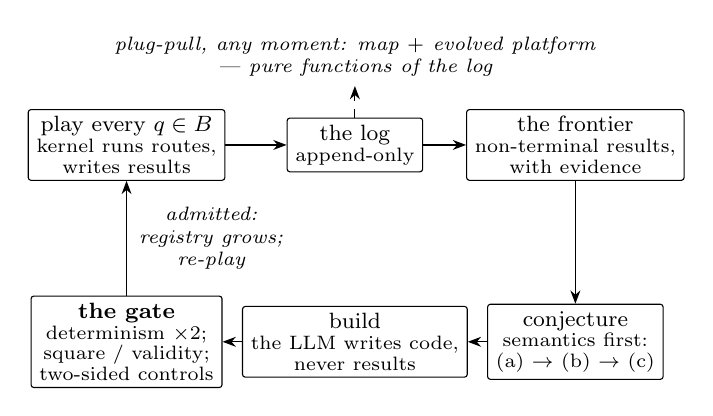
\begin{tikzpicture}[font=\footnotesize, >=Stealth,
  box/.style={draw, rounded corners=1pt, align=center,
              inner xsep=3pt, inner ysep=2.5pt},
  lab/.style={font=\scriptsize\itshape, align=center}]
  \node[box] (play) at (0,0) {play every $q \in B$\\[-2pt]
    \scriptsize kernel runs routes,\\[-2pt]\scriptsize writes results};
  \node[box] (log) at (2.9,0) {the log\\[-2pt]\scriptsize append-only};
  \node[box] (front) at (5.7,0) {the frontier\\[-2pt]
    \scriptsize non-terminal results,\\[-2pt]\scriptsize with evidence};
  \node[box] (conj) at (5.7,-2.5) {conjecture\\[-2pt]
    \scriptsize semantics first:\\[-2pt]
    \scriptsize (a) $\to$ (b) $\to$ (c)};
  \node[box] (build) at (2.9,-2.5) {build\\[-2pt]\scriptsize the LLM
    writes code,\\[-2pt]\scriptsize never results};
  \node[box] (gate) at (0,-2.5) {\textbf{the gate}\\[-2pt]
    \scriptsize determinism $\times 2$;\\[-2pt]
    \scriptsize square / validity;\\[-2pt]
    \scriptsize two-sided controls};
  \draw[->] (play) -- (log);
  \draw[->] (log) -- (front);
  \draw[->] (front) -- (conj);
  \draw[->] (conj) -- (build);
  \draw[->] (build) -- (gate);
  \draw[->] (gate) -- node[lab, right=1pt]
    {admitted:\\registry grows;\\re-play} (play);
  \draw[->, dashed] (log.north) -- +(0,4mm)
    node[above, lab] {plug-pull, any moment: map $+$ evolved
      platform\\--- pure functions of the log};
\end{tikzpicture}
\caption{One loop iteration, no valve. The LLM conjectures and
builds; only the kernel writes results, and only the gate writes the
registry. The conjecture order (a)--(c) is fixed:
semantics first, then syntax. Plug-pull is safe at any moment
because both exit deliverables regenerate from the append-only log
byte-identically, and best-per-question only ever improves.}
\label{fig:loop}
\end{figure}

\paragraph{The conjecture order}
Conjectures go \emph{semantics first, then syntax} --- this is the
vision's core discipline, and it is fixed, not a heuristic:
\begin{itemize}
\item[\textbf{(a)}] \textbf{new solving for existing languages} ---
  a new solver pair, a portfolio or budget policy, a certificate
  printer, a discharge engine: new \emph{decision procedures} first;
\item[\textbf{(b)}] \textbf{new translation} --- new pairs, new
  routes to existing solvers;
\item[\textbf{(c)}] \textbf{new languages} --- abstraction or
  specialization deltas, proposed only when a translation or solving
  move keeps winning ad hoc and reifying it would make the win
  reusable and cheap. New syntax is \emph{earned} by demonstrated
  semantics, never invented ahead of it.
\end{itemize}
The order is the previous design's closing insight made operational
(\cref{fig:unknowns}): the commuting square
$I_s(p) \equiv_\pi \Lambda(I_t(T(p)))$ relates four artifacts, and
given any three, the equation constrains the fourth. Each conjecture
class solves the square for a different unknown, and one gate
adjudicates all of them, because \emph{the gate checks the square,
not the artifact}: it never asks which slot the untrusted producer
filled.

\begin{figure}
\centering
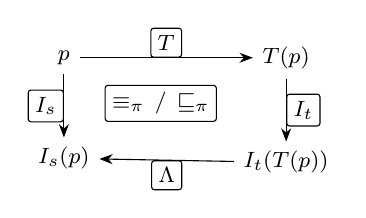
\begin{tikzpicture}[font=\footnotesize, >=Stealth,
  node distance=8mm and 22mm,
  slot/.style={draw, rounded corners=1pt, inner sep=2.5pt}]
  \node (p)  {$p$};
  \node[right=of p]  (tp) {$T(p)$};
  \node[below=of p]  (sb) {$I_s(p)$};
  \node[below=of tp] (tb) {$I_t(T(p))$};
  \draw[->] (p)  -- node[above, slot] {$T$} (tp);
  \draw[->] (p)  -- node[left, slot]  {$I_s$} (sb);
  \draw[->] (tp) -- node[right, slot] {$I_t$} (tb);
  \draw[->] (tb) -- node[below, slot] {$\Lambda$} (sb);
  \path (p) -- node[midway, slot] {$\equiv_\pi \,/\, \sqsubseteq_\pi$} (tb);
\end{tikzpicture}

\medskip
\footnotesize
\setlength{\tabcolsep}{3pt}
\begin{tabular}{@{}lll@{}}
\toprule
solves for & the discovered object & checked by \\
\midrule
(a) the procedure & a solver pair & result validity \\
(b) $T$ & a translation pair & the square, per run \\
(c) $\pi$ & an abstraction & the lax square \\
(c) $I_t$ & language $+$ parent pair & the square \\
--- $I_s$ & reverse-engineering & external anchor \\
\bottomrule
\end{tabular}
\Description{The commuting square with each artifact boxed, and a
table mapping each conjecture class to the unknown it solves for and
the check that adjudicates it.}
\caption{The conjecture order walks the square's unknowns, semantics
first. Solving for $I_s$ --- guessing the semantics of an existing
real-world language --- is the one inversion an internal check
cannot adjudicate; it stays anchor-bound and outside the loop. A new
language enters only as (c): stipulated semantics checked against a
parent the platform already trusts, adding nothing to the trusted
base.}
\label{fig:unknowns}
\end{figure}

\paragraph{One gate, no valve}
Whatever is built --- by the loop or by hand; manual registration is
the same path, human-invoked, no special case --- is admitted by one
check: determinism is \emph{measured} (every executable runs twice,
outputs byte-compared), the square or result validity is checked on
the entry's corpus, and \emph{two-sided controls} must hold --- the
intact artifact passes its vectors, and every supplied mutant fails,
because a checker that cannot be made to fail is unfalsifiable.
Admission evidence is stamped into the manifest by the checker,
never self-reported. The previous design held registration behind a
human valve; the kernel has none, and the reasoning is worth
stating. What the valve protected --- answer soundness --- is
protected by construction: existential certification bypasses route
trust entirely, universal certification is graded, and the LLM has
no code path to a result. What autonomy actually risks is registry
clutter, which the result order neutralizes (junk never wins a
best-per-question) and which pruning --- a human act between runs
--- can clean; during a run the registry only grows.

\paragraph{Plug-pull}
Stopping is safe at any moment: the driver checkpoints after every
result and every admission, and the exit deliverables are pure
functions of the log --- (i) the \emph{frontier summary}: best
result, route, and cost per question, the non-terminal results with
their evidence, and the delta since iteration zero (expanded or
not); (ii) if expanded, the \emph{evolved} \hg{}: the kernel
unchanged plus everything registered, with admission evidence. The
next benchmark starts from it, which is how maps compound.

\paragraph{Bootstrap from empty}
The kernel ships with zero languages and zero pairs, and everything
above must work on that instance --- the design's simplicity test.
Presented a benchmark, the LLM's first act is writing the root
language's interpreter (the trusted base, graded \emph{stipulated};
benchmark labels and supplied vectors are its only corroboration),
then a first naive solver pair, then growth. Grades bottom out at
\emph{claimed} until the registry holds a second lineage --- and the
map says so, which is the honesty rule doing its work on day one.

%% §5 — the facilitation theorems. Drafted in Phase 1, in lockstep
%% with mechanization/Calculus/Frontier.lean; Lean names are cited
%% inline, and a statement without a Lean name says where its content
%% lives instead. Sufficiency theorems first, necessity ablations
%% after, assumptions typeset as the theorems' TCB.

\section{Why this explores the frontier}
\label{sec:theorems}

An explorer of a frontier must satisfy six properties or it is not an
explorer: it must draw a map its untrusted explorer cannot falsify
(F1), never lose ground (F2), know at every open point what would
extend the map there (F3), eventually reach every point inside the
true frontier (F4), know when a survey is finished (F5), and work in
any territory (F6). This section states each as a theorem over the
model of \Cref{sec:problem}, with its proof burden placed honestly:
mechanized, reduced to a named assumption, or empirical. The model is
small on purpose --- a registry is a set of items, a candidate is a
list of items, and answerability is the filtration of
\Cref{def:answerable}; its two monotonicities (stages shrink along
conditions, grow along registries) carry F2--F5.

\begin{theorem}[F1, unfalsifiable map]
\label{thm:sound}
Whatever the generator of pairs does --- blind or adversarial ---
the map's labels are truthful: (i) every existential answer is true
at the source, assuming only adequacy of the source interpreter; (ii)
every universal answer carries exactly the assurance class,
direction, and trusted base computed by the componentwise meet of its
route's contracts --- labels never overstate, because meets never
exceed their arguments.
\end{theorem}

\noindent
This is the instrument's own theory, consumed as an interface: (i) is
witness replay (\textsf{existential\_self\_certifying}, axiom-free),
(ii) is the contract algebra
(\textsf{weakest\_link\_universal}, \textsf{Contract.comp\_glb},
\textsf{lax\_universal\_transfer})~\citep{hurdygurdy2026calculus}.
The residue is stated, not hidden: a false universal in the corner
where no branch corroborates and no anchor covers is not excluded by
theorem --- it is bounded empirically (measured escape rates,
negative controls) and shrunk by the trust loop, and the map records
per answer which corner it sits in.

\begin{theorem}[F2, monotone exploration]
\label{thm:monotone}
If $G \subseteq G'$ then every question answerable at $G$ is
answerable at $G'$
{\normalfont(\textsf{Frontier.answerable\_mono}, axiom-free)}; and,
by the pair-level ratchet
{\normalfont(\textsf{ratchet\_preserves\_faithful})}, every standing
verdict stands.
\end{theorem}

\begin{theorem}[F3, complete local gradient]
\label{thm:gradient}
For every question unanswerable at $G$: a first failing condition
exists {\normalfont(\textsf{diagnosis\_total})}, is unique
{\normalfont(\textsf{diagnosis\_unique})}, never regresses under
growth {\normalfont(\textsf{diagnosis\_progress})}, and strictly
advances under any \emph{adequate} extension --- one after which some
admitted candidate survives one condition further
{\normalfont(\textsf{diagnosis\_strict\_progress})}.
\end{theorem}

\noindent
Totality is where the model earns the word \emph{complete}: the five
conditions are exhaustive \emph{by construction}, because
answerability is defined as their conjunction
(\Cref{def:answerable}), so the demand taxonomy is a theorem input,
not a design choice. What the platform's diagnosis \emph{names} ---
that the returned generation target, if admitted, discharges the
failing condition --- is the specification of \texttt{why\_not}, met
by construction in the implementation; it enters the theorems only as
the adequacy hypothesis. The one classical step
(\textsf{diagnosis\_total}) is itself informative: an unanswerable
question does not name its obstacle constructively --- the platform
computes it because its five conditions are decidable.

\begin{theorem}[F4, the chain lemma]
\label{thm:chain}
Along any growing chain of registries in which every diagnosis is met
by an adequate extension, $N$ steps answer the question
{\normalfont(\textsf{adequate\_chain\_answerable})}: the diagnosis
index is bounded by $N$ and strictly increases, so it runs out of
room.
\end{theorem}

\begin{assumption}[Fair enumeration]
\label{ass:fair}
Every demanded target is eventually attempted: the books aggregate
demand, and a human --- or a scoped mandate --- eventually acts on
standing demand.
\end{assumption}

\begin{assumption}[Gate liveness]
\label{ass:gate}
A sound design with adequate evidence is eventually admitted: builders
eventually produce, and the gate does not reject forever, a pair
discharging a named requirement that some sound pair can discharge.
\end{assumption}

\begin{theorem}[F4, relative completeness]
\label{thm:complete}
Under \Cref{ass:fair,ass:gate}, every question answerable at some
finite extension of $G$ over the candidate universe is eventually
answered by the loop.
\end{theorem}

\noindent
The mathematical content is \Cref{thm:chain}; the assumptions supply
its chain, and they are the theorem's honest trusted base --- both
are what the automation pipeline exists to provide, and both are
measured (queue throughput, gate escape rates) rather than provable.
The framing is deliberately that of relative
completeness~\citep{cook1978soundness}: complete relative to the
candidate universe and the domain's supply, not an oracle claim ---
undecidability, the adequacy floor of the source semantics, and the
finite anchor supply stand at every registry size.

\begin{theorem}[F5, saturation is a decidable, reachable fixpoint]
\label{thm:saturation}
For a pinned finite benchmark and a finite known set, the saturation
predicate of \Cref{def:saturation} is computable from the books ---
an emptiness check on the derived tier-2 set --- and the loop
restricted to in-set targets reaches it in finitely many iterations:
target signatures are finitely many, an admitted signature cannot
recur (dedup plus the ratchet), and each iteration retires at least
one.
\end{theorem}

\noindent
The finite-pool argument --- admitted signatures never recur, and
form a duplicate-free subset of the pool, so admissions run out of
room --- is mechanized as
{\normalfont\textsf{saturation\_terminates}}. The decidability half
is the implementation's contract: saturation is an exit code, not a
judgment.

\begin{theorem}[Currency: the status ratchet; conditional plans]
\label{thm:currency}
(i) Along any lifecycle a pair's tier only advances and its evidence
payload only accumulates
{\normalfont(\textsf{lifecycle\_ratchet}, axiom-free)}: a built pair
still carries the demand that created it. (ii) A mixed route's
conditional contract (\Cref{def:conditional}) is a lower bound on its
realized contract once every frontier hop is discharged by a pair
whose achieved contract dominates its requirement
{\normalfont(\textsf{conditional\_plan\_sound}, via monotonicity of
the meet)}: conditional plans never overpromise.
\end{theorem}

\begin{theorem}[F6, domain-genericity]
\label{thm:generic}
F1--F5 are stated and proved over the domain signature alone ---
abstract languages, items, conditions, contracts --- so they transfer
to any domain by instantiation. What does not transfer for free is
the supply side, and \Cref{sec:kit} states it as the explicit
obligation: the theorems are conditional on the kit, and the books
measure the condition.
\end{theorem}

\paragraph{Necessity: the ablations}
Each load-bearing feature of the instrument is needed for a specific
theorem, and dropping it breaks that theorem --- which is the precise
sense in which the current platform is the means to this paper's end.
Without \emph{determinism}, a square check cannot distinguish defect
from coin flip and F1(i)'s replay proves nothing. Without the
\emph{ratchet}, F2 fails and the curve can regress; a map that can
silently shrink is not a map. Without \emph{typed aborts} and the
fixed diagnosis order, the filtration of \Cref{def:answerable} has no
well-defined first failure and F3 degenerates to blind enumeration.
Without the \emph{existential/universal asymmetry} --- replay for
witnesses, graded meets for universals --- an untrusted generator
forges map entries and F1 falls adversarially. Without \emph{pinned
ingestion}, ``the benchmark'' is not a fixed set and F5's fixpoint is
not defined. And without the \emph{human valve} (or its mandate
generalization, which preserves it), \Cref{ass:fair}'s enumeration
has no scope and the books no meaning: demand-driven growth
presupposes someone accountable for what counts as demand.

\paragraph{The trusted base, collected}
F1(i) assumes source-interpreter adequacy; F1(ii)'s corner is
empirical; F4 assumes \Cref{ass:fair,ass:gate}; F5 assumes the pin
and the finiteness of the known set; F6 defers the supply side to the
kit. Nothing else is assumed, and each assumption is either measured
by the platform's own books or discharged by construction in the
implementation --- the reader can locate every claim's burden, which
is the property the whole architecture is built to have.

%% §6 — written out in Phase 4: the kit frozen (K1–K4 named here, the
%% definition site — INVERSION.md cites this vocabulary), the design
%% oracle, the atlas (O1), challenge bundles, and the pre-registered
%% protocol. The campaign it pre-registered has run; §7 (status.tex)
%% summarizes it. No measurements appear in this section, by design.

\section{The domain kit, and the far side as a design oracle}
\label{sec:kit}

\subsection{The kit}
\label{sec:kit-list}

Pointing the explorer at a domain costs exactly four things, and the
theorems of \Cref{sec:theorems} are conditional on them — this list is
the instantiation obligation of F6, frozen. Each item is named, so that
this paper and the platform's design documents cite one vocabulary; and
each is stated with what its absence costs, so a domain can read off
exactly which guarantee it forfeits by not supplying it:

\begin{enumerate}
\item[\textbf{K1}] \textbf{A reasoning hub}: at least one language a
  mechanized decision procedure consumes directly, with declared
  question shapes and declared budgets. (Without it, no question clears
  the shape and cost conditions.)
\item[\textbf{K2}] \textbf{Deterministic shared interpreters} for every
  language touched, exposing named observables. (Without them, squares
  cannot be checked and F1's replay proves nothing.)
\item[\textbf{K3}] \textbf{At least one external semantic anchor}, if
  trust beyond per-run checking is wanted. (Without it, the trust axis
  saturates at \textit{checked}; the theorems still hold, and the map
  says so.)
\item[\textbf{K4}] \textbf{A pinned benchmark}: a finite question set
  with recorded provenance. (Without the pin, F5's fixpoint is not
  defined.)
\end{enumerate}

\noindent
K3 is the one graded \emph{optional}, and the shape of its grading is
the kit's own discipline in miniature: an absent optional obligation is
a \emph{recorded ceiling}, never a silent failure.

The kit is deliberately mundane: hardware model checking supplies all
four today; C program analysis supplies them down a longer spine; and
the platform's own field-blind corners (chemical reaction networks,
molecular notation) are the cheap existence proof that nothing in the
list assumes computation-adjacent
languages~\citep{hurdygurdy2026calculus}.

\subsection{The far side as a design oracle}
\label{sec:kit-oracle}

A terminal board is not a failure list. By the honest-failure
discipline, every open question carries typed evidence, and each
obstacle class comes with an \emph{extraction operator} turning that
evidence into the specification of the missing instrument:

\begin{center}
\footnotesize
\setlength{\tabcolsep}{3pt}
\begin{tabular}{@{}lll@{}}
\toprule
obstacle & evidence & extraction operator \\
\midrule
shape & blocked $\varphi$s verbatim & fragment hull + atlas \\
charted shape & hull + census slice & procedure-synthesis brief \\
cost & cost curves at the wall & binding-parameter fit \\
cost (abstraction) & the spurious corpus & separating predicates \\
trust & uncorroborated verdicts & certificate + anchor joins \\
outside the closure & the wall itself & in-closure relaxation \\
\bottomrule
\end{tabular}
\end{center}

Four operators are already mechanical:

\begin{itemize}
\item The \emph{binding-parameter fit} is the report's failure-mode
  reading: blocked instances get their cost curves measured by an
  ascending probe, and the fit classifies --- exponential in the
  unrolling bound means deeper search will not close it (demand an
  unbounded engine or a property transformation); linear means depth
  is affordable (raise the budget before demanding an instrument).
\item The \emph{atlas location}: a registry-side reference table of
  the known decidability landscape, so a shape-blocked demand
  arrives locating itself --- the setting in which its shape is
  decidable, the procedure family that decides it natively, and the
  \emph{known crossing}, the classical reduction that would
  discharge it on an existing hub instead of a new logic
  (liveness-to-safety; self-composition for 2-safety; monitor
  weaving for temporal shapes). The atlas is reference data,
  protected like every instrument the gate trusts; a shape it does
  not know reads \textit{uncharted}, never a guess. Chartedness is
  load-bearing: it classifies a procedure demand as instantiation
  (inside the known set, blocking saturation) or discovery (outside,
  on the frontier).
\item The \emph{scout} measures before anyone designs: candidate
  embeddings for a blocked shape are prototyped and their encoding
  blowup measured, so a procedure demand arrives justified by
  numbers rather than taste.
\item The \emph{procedure-synthesis brief} turns a charted
  procedure demand into a self-contained work item: the
  fragment hull of its citing $\varphi$s, the atlas location and
  family, the required contract, the census slice that will falsify
  the build, and the certificate obligation.
\end{itemize}

\noindent
The recommender is audited in kind --- every recommendation is a
prediction of closure, checked ex post against realized closure ---
and the remaining operator (separating predicates mined from the
persistent spurious corpus) is named work, staged behind the same
shadow discipline as every other delegated judgment.

\paragraph{Challenge bundles}
Frontier pairs are exportable: a board entry carries pinned citing
questions, declared budgets, a required contract, and the near side's
baseline census — a self-contained challenge for the domain's solver
community. This is the sense in which the map's far side is a demand
oracle for the ecosystem: competitions supply benchmarks to the
platform; terminal boards supply open problems, with evidence counts,
back.

\subsection{The pre-registered protocol}
\label{sec:kit-protocol}

This paper was written with no benchmarks section, its place held by
the following protocol, pre-registered before any campaign ran ---
which is what keeps the reporting honest. The protocol has since run
its first campaign; \Cref{sec:status} summarizes where it stands,
and the full report regenerates byte-identically from the deposited
ledger.

\textbf{The benchmark.} The hardware model-checking competition
corpus (HWMCC~\citep{niemetz2018btor2}): designed by others, labeled,
native to the platform's bit-level hub — no translation debt to pay
before the loop starts. Ingestion is streamed-with-pin from a
community mirror at a fixed commit, every instance sha256-pinned; the
campaign starts from the already-pinned slice and widens by families,
one pinned extension at a time. The natural second act is software
verification (SV-COMP~\citep{beyer2021svcomp}) down the full
C-to-solver spine.

\textbf{The protocol.} (1) Pin the suite; establish ground truth
where labels exist. (2) Run the loop's player over every question,
books on, \textit{origin=campaign}, suite-tagged — manufactured
demand is displayed apart from organic demand by construction.
(3) What answers, answers with its way-census; what does not lands on
the books with its first failing obstacle, and blocked instances get
their cost curves measured. (4) Derive the board; promote what a
human (or, when earned, a mandate) registers; build, gate, merge.
(5) Re-run. The ratchet makes the curve monotone; stop at the
fixpoint, which is an exit code.

\textbf{Declared caps.} Unrolling bound, wall-clock and memory per
decide, instance count per iteration, one instance in memory at a
time; all caps ride in every result's provenance, and capped results
are labeled capped, never implied full-suite.

\textbf{Pre-registered honesty.} The curve may plateau on cost; the
plateau is a finding — the measured practice-frontier of the domain —
not a failure. \textit{unknown} and \textit{resource-out} are
counted, never hidden. A terminal board dominated by frontier-only
entries is a \emph{successful} saturation. The tooling (the loop
driver, the saturation checker, the report generator, the promotion
command) is built and tested; the only numbers in this paper are
those of \Cref{sec:status}, each read from the deposited ledger.

%% §7 — exactly the experiments the paper rests on: the campaign that
%% forced the redesign (numbers read from the deposited ledger under
%% ../results/hwmcc-sosylab-beem/) and the kernel demonstration
%% (runs/btor2-demo/ in the repository).

\section{The experiments this paper rests on}
\label{sec:status}

Two experiments substantiate this paper: the campaign that forced
the redesign, and the redesigned platform's first demonstration.
Nothing else is claimed.

\paragraph{The campaign that forced the redesign}
The previous design ran a pre-registered protocol to completion:
seven loop iterations over the pinned 110-question
\texttt{hwmcc-sosylab-beem} suite~\citep{niemetz2018btor2}, every
instance sha256-pinned, the ledger deposited in the repository and
the full report regenerating from it byte-identically. The outcome,
read from the ledger: 82 of 110 questions answered at least once and
never receded; four proved at every depth; every verdict agreed with
every external label; and, after the host's engine enumeration
closed, exactly \emph{one} surviving demand entry --- \emph{build a
better unbounded engine} --- with 29 citing questions. The
structural lesson mattered more than the numbers: every artifact the
loop could admit was meaning-preserving by construction, so the loop
was \emph{conservative over truth} --- seven iterations of a
discovery loop produced instruments, never facts, and its one demand
was exogenous. That ceiling, together with the judgment that the
demand machinery had grown past its justification, is what
\cref{sec:intro} designed away from.

\paragraph{The kernel, demonstrated by carry-over}
The redesign's first test is the previous platform itself: Era-3
code is not discarded but \emph{mined} --- wrapped in kernel
manifests and re-certified through the gate it must now pass. The
first slice is the BTOR2 interpreter (vectors from the existing test
suite; a semantics-blind mutant as negative control) and the
\texttt{btormc} solver pair (bounded model checker; witness
carry-back; an always-\textit{all} mutant; the canary discipline
carried over: silent exhaustion is trusted only after the binary
answers \textit{sat} on a trivially reachable input). Both admitted:
vectors pass, every mutant fails, determinism measured twice. The
demonstration benchmark then plays three questions through the
kernel, and its map is worth reading in full because every row
exercises a different part of the design:

\begin{center}
\footnotesize
\setlength{\tabcolsep}{4pt}
\begin{tabular}{@{}lllll@{}}
\toprule
question & ask & best result & grade & status \\
\midrule
counter-reach & $\exists$, $k{=}20$ & witness, depth 5 & replayed &
  terminal \\
frozen-unreach & $\forall$, $k{=}20$ & all(20) & claimed &
  terminal \\
frozen-unreach & $\forall$, $\infty$ & all(20) & claimed &
  \textbf{frontier} \\
\bottomrule
\end{tabular}
\end{center}

\noindent
The witness was solved at the target, carried back, and replayed
through the source interpreter --- terminal at the rung trust cannot
raise or lower. The bounded universal is terminal but graded
\emph{claimed}, exactly as strong as its evidence: \texttt{btormc}
prints no certificate, and the ladder says so rather than rounding
up. And the unbounded ask sits honestly on the frontier at
$\textit{all}(20)$, carrying its route and evidence --- the
campaign's structural finding reproduced in miniature, and the first
conjecture the order of \cref{sec:loop} licenses is class (a): a
second solver pair, an unbounded engine, whose disjoint lineage
would also light \emph{corroborated} for the bounded row. The
remaining carry-over --- thirteen languages, fifteen translation
pairs, ten solver backends --- is named work, deliberately of the shape the
loop itself performs, and it is the redesign's standing experiment:
whether the conjecture order, fed by frontier evidence alone,
reconstructs and then extends what the previous generation built by
hand.

%% §8 — the discovery program: INVERSION.md distilled to paper scale.
%% Everything here is named work, deliberately marked as such; the
%% landed machinery it leans on is cited where it is leaned on. The
%% repository document carries the full argument and the code-level
%% seams.

\section{Beyond cartography: the square's other unknowns}
\label{sec:vision}

\Cref{sec:status} ends at a ceiling: the loop can discover
\emph{instruments}, never \emph{facts}. Nothing in the ledger has a
shape that could hold a discovered truth, because the only currency
is capability, and every demand a terminal board can voice is
exogenous good news the loop cannot itself supply. This section
states the one structural change that lifts the ceiling, and what
follows from it. Everything in it is staged design --- named work
with its landed seams cited --- not a claim of results.

\paragraph{One equation, four unknowns}
The platform is one equation solved for one unknown. The square
$I_s(p) \equiv_\pi \Lambda(I_t(T(p)))$ relates four artifacts ---
source semantics $I_s$, target semantics $I_t$, translation $T$,
projection $\pi$ (with its reading map $\Lambda$) --- and given any
three, the equation constrains the fourth
(\Cref{fig:inversions}). Every registered pair, every builder run,
every gate check solves for $T$. Solving for $\pi$ --- the coarsest
projection under which the square still commutes --- is
abstract-domain discovery, checked by the lax square exactly as
today's abstraction pairs are. Solving for $I_t$ --- an interpreter
for a \emph{new} target --- is a \emph{stipulated} semantics, checked
against the fixed $I_s$. Solving for $I_s$ is semantic
reverse-engineering of an existing language, and it is the one
inversion that is anchor-bound (below). The reason this is a small
change rather than a new architecture: \textbf{the gate checks the
square, not the artifact}. Coverage, determinism, two-sided negative
controls --- none of it asks which slot the untrusted producer
filled, and the square is stated over the domain signature alone, so
all four inversions inherit F6's genericity.

\begin{figure}
\centering
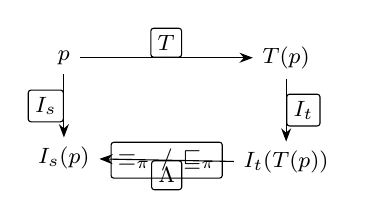
\begin{tikzpicture}[font=\footnotesize, >=Stealth,
  node distance=8mm and 22mm,
  slot/.style={draw, rounded corners=1pt, inner sep=2.5pt}]
  \node (p)  {$p$};
  \node[right=of p]  (tp) {$T(p)$};
  \node[below=of p]  (sb) {$I_s(p)$};
  \node[below=of tp] (tb) {$I_t(T(p))$};
  \draw[->] (p)  -- node[above, slot] {$T$} (tp);
  \draw[->] (p)  -- node[left, slot]  {$I_s$} (sb);
  \draw[->] (tp) -- node[right, slot] {$I_t$} (tb);
  \draw[->] (tb) -- node[below, slot] {$\Lambda$} (sb);
  \path (sb) -- node[midway, slot] {$\equiv_\pi \,/\, \sqsubseteq_\pi$} (tb);
\end{tikzpicture}

\medskip
\footnotesize
\setlength{\tabcolsep}{3.5pt}
\begin{tabular}{@{}lll@{}}
\toprule
solve for & the discovered object & checked by \\
\midrule
$T$ & a translation --- \emph{the platform today} & the square, per run \\
$\pi$ & an abstract domain & the lax square \\
$I_t$ & a stipulated semantics (new target) & the square, vs.\ fixed $I_s$ \\
$I_s$ & semantic reverse-engineering & an external anchor (K3) \\
\bottomrule
\end{tabular}
\Description{The commuting square with each of its four artifacts
boxed, and a legend table mapping each unknown to the object
discovered by solving for it and to the check that adjudicates it.}
\caption{The commuting square has four unknowns, and each boxed slot
is a discovery mode: given any three artifacts, the equation
constrains the fourth, and the same gate falsifies a candidate in
any slot because the gate checks the square, not the artifact. Only
the $I_s$ inversion needs an external anchor; the other three are
checked against artifacts the platform already trusts.}
\label{fig:inversions}
\end{figure}

\paragraph{The ladder, and why its order is forced}
The inversions stage into a ladder in which \emph{each level's
checker is the previous level's product}:

\begin{center}
\footnotesize
\setlength{\tabcolsep}{2.5pt}
\begin{tabular}{@{}llll@{}}
\toprule
 & object discovered & producer & checker \\
\midrule
L0 & routes, translations & LLM builder & the square (\emph{landed}) \\
L1 & properties $\varphi$ & LLM proposer & \texttt{decide} at a hub \\
L2 & vocabularies & mining over L1 & leverage over the board \\
L3a & transfer functions & LLM proposer & the lax square \\
L3b & the fixpoint procedure & builder lane & L3a + solver gate \\
\bottomrule
\end{tabular}
\end{center}

L1's interestingness is measured against a saturated board, which
requires L0 to have run to its fixpoint; L2 mines the population of
properties that survived L1; L3a's lax square is checked against a
concrete semantics reached through registered pairs; L3b inherits
its soundness from L3a. One consequence matters more than the rest:
the platform's design line escalates any target whose design needs a
creative act, so ``invent a decision procedure for this fragment''
escalates under every mandate, permanently and correctly --- but
``compute the fixpoint over \emph{this} vocabulary'' is mechanical.
\textbf{Discovering the language first is what moves the algorithm
across the design line} --- the exact sense in which languages and
properties are a load-bearing prerequisite for semantics and
algorithms, not merely a natural order of study.

\paragraph{L1: properties as searched objects}
A question is $(p, \varphi)$; today both arrive from outside and the
loop searches over routes. Making $\varphi$ the searched object over
a fixed population needs no new grammar: a hub already declares the
question shapes it consumes (K1), and that declaration \emph{is} the
space of proposable conjectures --- the LLM proposes syntax in a
declared grammar, the hub decides truth. The two standing objections
to property mining are both mechanical here, which is what makes the
level admissible under the platform's honesty rules: a proposed
$\varphi$ is \emph{novel} iff $F \not\models \varphi$ for the
accumulated fact set $F$ (one query), and \emph{useful} iff assuming
$\varphi$ closes a question standing on the terminal board ---
measured directly against the open set, e.g.\ the 29 blocked pins of
\Cref{sec:status}. Verdicts deposit into a \emph{fact ledger} beside
the demand ledger, under two non-negotiable disciplines. A deposit
is \emph{graded, never believed}: it enters later answers as an
assumption, so it carries certificates re-discharged by an engine of
disjoint declared lineage, and a lemma-carrying answer's assurance
is the meet including its weakest cited fact. And a deposit is
\emph{not a demand}: conjectures are an infinite pool, so if they
counted toward in-set demand, saturation would never terminate and
F5 would break --- the fact ledger stays outside the fixpoint, and
the discovery loop terminates on a declared proposal budget that
rides in provenance like every other cap. A proposed $\varphi$ the
hub cannot decide within budget is not waste but a \emph{conjecture
with a cost obstacle}: a second kind of open board entry, carrying a
bound (``holds to $k{=}20$'') rather than a probability --- the
literal form of new unproven properties, and a deliverable no
current pipeline produces.

\paragraph{L2: vocabularies --- the honest sense of a new language}
Language \emph{invention} stays refused: registration is the human
valve, and a language is the deepest trusted artifact in the
calculus. What is discoverable is narrower and clears the membership
rule without argument: a \emph{vocabulary} --- a finite set of
predicate templates over the hub's declared grammar, its interpreter
deterministic and one line. That is a formal language in exactly the
sense intervals, octagons, and polyhedra are formal languages; the
platform's registered interval domain is the landed proof that such
a domain rides the pair machinery unchanged. The difference the loop
makes is that intervals were \emph{designed} and this vocabulary is
\emph{mined}: the recurring templates in the property population
that survived L1, ranked by measured leverage over the board. The
fragment atlas grows a third tier for it --- \emph{charted},
\emph{uncharted}, \emph{discovered} --- so the next benchmark
classifies against what this one mined and discoveries compound.

\paragraph{L3: the fixpoint is the procedure}
Given a mined vocabulary, its transfer functions --- how each source
construct moves a predicate to a predicate --- are a stipulated
semantics, checked as a lax square with the direction axis the
platform already carries: universal verdicts transfer down the
$\sqsubseteq$, existentials replay, and a spurious witness is a
refinement demand. The algorithm that saturates those transfer
functions over an artifact \emph{is} a decision procedure for the
fragment, and its epistemic status is the payoff of this route over
direct synthesis: census replay is testing --- a candidate that
agrees with 110 corroborated verdicts may be wrong on the 111th ---
but \textbf{a fixpoint over a checked domain is sound by
construction}, its correctness following from the lax square rather
than from agreement on a corpus. The discovered procedure clears the
solver gate \emph{besides}, not \emph{instead}: same gate, strictly
better prior. One extension is mandatory: a vocabulary mined from a
corpus decided by engine $E$ is not independent of $E$, so the
lineage declaration must carry mining provenance, or corroboration
between a discovered procedure and the engine that taught it is
fiction.

\paragraph{The anchor ceiling, and the door in it}
F1(i) assumes source-interpreter adequacy: the shared interpreters
(K2) are the trusted base, and an LLM generating $I_s$ would put the
producer \emph{inside} it, collapsing the central asymmetry. The
only defence is an external anchor (K3), and anchors exist in small
finite supply --- so the $I_s$ inversion is real, useful, and
permanently rate-limited. The door is that \textbf{a new object has
nothing to be adequate to}: a mined vocabulary, its transfer
functions, a discovered procedure's state space are formalizations
of nothing in the world, so their semantics is stipulated and every
remaining question is internal and checkable --- does the square
commute, is the abstraction sound, does the fixpoint decide the
fragment. The L1--L3 pathway is therefore anchor-free while the
$I_s$ inversion is not, which is the whole reason to prefer it. At
field scale this is the shape of abstract interpretation as a
discipline --- domains stipulated and proved sound against a
concrete semantics, never a concrete semantics guessed --- with the
mining and the checking moved into a loop.

\paragraph{What it costs the theorems}
The model of \Cref{sec:theorems} is deliberately small --- a
registry is a set of items, a candidate is a list of items --- and a
deposited fact \emph{is} an item: using it as a lemma is
composition. So F2--F5 apply to discovery with zero new proof
burden, and F1(ii)'s meet already prices a lemma-carrying answer.
The seventh theorem is then an obligation rather than a leap:

\begin{theorem}[F7, unfalsifiable deposit --- stated, not yet
mechanized]
\label{thm:deposit}
Whatever the proposer does --- blind or adversarial --- every entry
in the fact ledger is truthful, and every answer citing one carries
exactly the assurance computed by the componentwise meet over its
route and its cited facts.
\end{theorem}

\noindent
The burden sits where F1's does: the fail-safe direction is the
certificate schema's defining property --- any counter-model refutes
the \emph{candidate}, never the answer; the platform's invariant
re-discharge seam is the landed instance --- and the grading is the
existing meet over a widened item set. The residue is the corner
F1(ii) already states: a deposit no independent lineage
re-discharges is \emph{reproducible}, not \emph{proved}, and the
books say which. What discovery charges a domain is a second,
conditional kit --- the frozen kit of \Cref{sec:kit-list} stays
frozen, and nothing is retroactively demanded of a domain that wants
cartography only:

\begin{enumerate}
\item[\textbf{K5}] \textbf{A proposable question grammar}: K1's
  declared shapes made generable, not merely recognizable. (Without
  it there is no candidate space; L1 cannot start.)
\item[\textbf{K6}] \textbf{Decidable relative entailment},
  $F \models \varphi$ over the accumulated facts --- needs the hub's
  fragment closed under conjunction and negation. (Where it fails it
  degrades: novelty falls back to a syntactic filter plus measured
  leverage, and the map records which mode was used.)
\item[\textbf{K7}] \textbf{A certificate schema} for at least one
  universal verdict class --- \emph{optional}. (Without it,
  discovery runs existential-side only and the axis saturates at
  \emph{existential}, with the map saying so --- exactly as trust
  saturates at \emph{checked} without K3.)
\end{enumerate}

\paragraph{The genericity control}
The cheapest falsification of every claim above is already in the
tree: the platform's chemical-reaction-network pair reduces
discrete-population CRNs to \textsf{QF\_LIA} bounded reachability
--- a hub with no program anywhere near it. Its kit census is honest
and one item short: K1, K2, K5, K6, K7 hold; \textbf{K4 does not}
--- no pinned CRN suite exists, and ingesting one is the
experiment's prerequisite and its only part not already in the tree.
With the pin in hand, run L1 over it: propose $\varphi$ over species
populations, decide at the SMT hub, filter by relative entailment,
measure leverage against that suite's board. If the loop needs one
line of program-specific code, domain-independence is false and
found out cheaply. If it does not, the deposit is a discovery result
in chemistry produced by an architecture that was never told what a
molecule is.

\paragraph{Where the wall stands}
Unmoved. Nothing here crosses the four walls of
\Cref{sec:conclusion}: inversion does not push the frontier of
reducible decidability --- it populates the region \emph{behind} the
frontier with content, and supplies one new way to produce the
instruments that push it. Nor does any of it put semantics into a
model: the LLM remains a syntax engine permanently --- that is the
design, not a concession, and it is what keeps the producer safely
untrusted. What the platform supplies is a \emph{semantic
adjudicator with memory}: deterministic, per-artifact, and ---
the part no benchmark, score, or reward model has ---
\emph{depositing}, so the syntax that survives adjudication
accumulates as checked artifacts the next question inherits and the
ratchet never surrenders. An LLM with a benchmark gets a score; with
a reward model, a gradient; with this, a growing registry of
artifacts whose meaning has been adjudicated one at a time ---
translations today; abstractions and stipulated semantics reachable
and anchor-free; reverse-engineered real-world semantics
anchor-bound, and honestly walled. The saturation fixpoint is the
phase transition at which the loop stops being able to find new
routes and starts being able to find new facts.

%% §8 — related work, compressed for the kernel re-cut.

\section{Related work}
\label{sec:related}

\paragraph{Decidability by reduction}
Answering a question by carrying it to a decision procedure is a
classical discipline, from quantifier
elimination~\citep{presburger1929,tarski1951decision} and
interpretations that transfer decidability between
theories~\citep{tarski1953undecidable,rabin1969trees} to
verification practice, where the move is institutional: bounded
model checking reduces to SAT~\citep{biere1999bmc}, theory
combination composes procedures~\citep{nelson1979simplification},
intermediate verification languages pipeline programs to
SMT~\citep{barnett2005boogie,filliatre2013why3}, and Ivy makes
landing in a decidable fragment the design objective
itself~\citep{padon2016ivy,padon2017epr}. Each strand fixes the
reduction and asks what it decides; \hg{} makes the evolving, gated
set of reductions the object of study, with budgeted cost inside
the definition and the boundary --- the frontier of non-terminal
results --- as the deliverable.

\paragraph{Single-edge theories, abstraction, certificates}
Certified compilation~\citep{leroy2009compcert,kumar2014cakeml} and
translation
validation~\citep{pnueli1998tv,necula2000tv,lopes2021alive2} are
statements about one translation; the companion
calculus~\citep{hurdygurdy2026calculus} develops the graph-level
theory this paper consumes, and the kernel's move is to run the
graph as an explorer. Abstract
interpretation~\citep{cousot1977abstract} supplies the lax half of
the directional square, and CEGAR~\citep{clarke2000cegar} the shape
of the refinement loop --- with the structural difference that
refinements are registered, reusable pairs and spurious
counterexamples persist as frontier evidence. Proof-carrying
code~\citep{necula1997pcc}, certifying
algorithms~\citep{mcconnell2011certifying}, verification
witnesses~\citep{beyer2015witnesses}, and checked proof
formats~\citep{wetzler2014drat,tan2021cakelpr} supply the trust
vocabulary; the grade ladder adds that the \emph{absence} of a
certificate is data --- a claim graded \emph{claimed} is a standing
demand for the printer and discharge engine that would upgrade it.

\paragraph{Competitions; conjecture generation}
HWMCC~\citep{niemetz2018btor2} and SV-COMP~\citep{beyer2021svcomp}
rank solvers on fixed benchmarks; the loop inverts the roles --- the
benchmark is fixed and the \emph{instrument grows}, the frontier
exported as evidence-carrying open problems. Automated
conjecture-making~\citep{fajtlowicz1988graffiti,colton2002hr} and
theory exploration~\citep{claessen2010quickspec} filter candidates
syntactically or statistically; here the LLM proposes only code and
conjectures, and a deterministic kernel adjudicates every claim by
running it --- the producer stays a syntax engine, permanently, and
that is the design rather than a concession.

%% §9 — re-cut 2026-08-06: the walls, the claim, the program.

\section{Limitations and conclusion}
\label{sec:conclusion}

Three walls stand at every registry size, and the design is drawn up
to them, not past them. \emph{Computability}: a route re-expresses a
question, never changes its degree; unbounded universal claims rest
on certificates, and without one they are bounded claims under
declared bounds, labeled so. \emph{Trust supply}: capability scales
with generated pairs, but the trusted base is the root interpreters,
graded stipulated until corroborated --- and independent lineages,
like external anchors before them, exist in finite supply, so the
grade ladder records where trust saturates rather than pretending it
does not. \emph{Cost}: deciding is exponential in the worst case
everywhere that matters; budgets are permanent provenance, capped is
labeled capped, and a frontier that stops moving under a fixed
registry is a finding --- the measured practice-frontier of that
registry --- not a failure.

Within the walls, the claim is deliberately modest in kind: an
architecture in which one edge kind carries both translation and
solving, one gate admits everything, one currency --- the result ---
holds both progress and failure, and one small proved kernel writes
every entry, so that an autonomous, untrusted LLM can grow the
instrument and play it without any answer resting on its word. The
previous generation of the platform is the first content of the new
one, re-certified through the gate; the standing experiment is
whether the conjecture order --- procedures, then translations, then
languages; semantics first, then syntax --- fed by frontier evidence
alone, reconstructs what was built by hand and then builds what was
not. The loop turns until the player stops cranking; what remains is
the map and the evolved instrument, and the next benchmark starts on
the ground the last one won. The vision is the means. The map is the
end.


\begin{acks}
This work was co-funded by the Czech Science Foundation under Grant
No.~23-07580X and the European Union under the project Robotics and
Advanced Industrial Production
(reg.~no.~CZ.02.01.01/00/22\_008/0004590).
\end{acks}

\bibliographystyle{ACM-Reference-Format}
\bibliography{../references}

\end{document}
